\chapter{In the Lucern Patch}

Our readers must now allow us to transport them again to the enclosure
surrounding M. de Villefort’s house, and, behind the gate, half
screened from view by the large chestnut-trees, which on all sides
spread their luxuriant branches, we shall find some people of our
acquaintance. This time Maximilian was the first to arrive. He was
intently watching for a shadow to appear among the trees, and awaiting
with anxiety the sound of a light step on the gravel walk.

At length, the long-desired sound was heard, and instead of one figure,
as he had expected, he perceived that two were approaching him. The
delay had been occasioned by a visit from Madame Danglars and Eugénie,
which had been prolonged beyond the time at which Valentine was
expected. That she might not appear to fail in her promise to
Maximilian, she proposed to Mademoiselle Danglars that they should take
a walk in the garden, being anxious to show that the delay, which was
doubtless a cause of vexation to him, was not occasioned by any neglect
on her part. The young man, with the intuitive perception of a lover,
quickly understood the circumstances in which she was involuntarily
placed, and he was comforted. Besides, although she avoided coming
within speaking distance, Valentine arranged so that Maximilian could
see her pass and repass, and each time she went by, she managed,
unperceived by her companion, to cast an expressive look at the young
man, which seemed to say, “Have patience! You see it is not my fault.”

And Maximilian was patient, and employed himself in mentally
contrasting the two girls,—one fair, with soft languishing eyes, a
figure gracefully bending like a weeping willow; the other a brunette,
with a fierce and haughty expression, and as straight as a poplar. It
is unnecessary to state that, in the eyes of the young man, Valentine
did not suffer by the contrast. In about half an hour the girls went
away, and Maximilian understood that Mademoiselle Danglars’ visit had
at last come to an end. In a few minutes Valentine re-entered the
garden alone. For fear that anyone should be observing her return, she
walked slowly; and instead of immediately directing her steps towards
the gate, she seated herself on a bench, and, carefully casting her
eyes around, to convince herself that she was not watched, she
presently arose, and proceeded quickly to join Maximilian.

“Good-evening, Valentine,” said a well-known voice.

“Good-evening, Maximilian; I know I have kept you waiting, but you saw
the cause of my delay.”

“Yes, I recognized Mademoiselle Danglars. I was not aware that you were
so intimate with her.”

“Who told you we were intimate, Maximilian?”

“No one, but you appeared to be so. From the manner in which you walked
and talked together, one would have thought you were two school-girls
telling your secrets to each other.”

“We were having a confidential conversation,” returned Valentine; “she
was owning to me her repugnance to the marriage with M. de Morcerf; and
I, on the other hand, was confessing to her how wretched it made me to
think of marrying M. d’Épinay.”

“Dear Valentine!”

“That will account to you for the unreserved manner which you observed
between me and Eugénie, as in speaking of the man whom I could not
love, my thoughts involuntarily reverted to him on whom my affections
were fixed.”

“Ah, how good you are to say so, Valentine! You possess a quality which
can never belong to Mademoiselle Danglars. It is that indefinable charm
which is to a woman what perfume is to the flower and flavor to the
fruit, for the beauty of either is not the only quality we seek.”

“It is your love which makes you look upon everything in that light.”

“No, Valentine, I assure you such is not the case. I was observing you
both when you were walking in the garden, and, on my honor, without at
all wishing to depreciate the beauty of Mademoiselle Danglars, I cannot
understand how any man can really love her.”

“The fact is, Maximilian, that I was there, and my presence had the
effect of rendering you unjust in your comparison.”

“No; but tell me—it is a question of simple curiosity, and which was
suggested by certain ideas passing in my mind relative to Mademoiselle
Danglars——”

“I dare say it is something disparaging which you are going to say. It
only proves how little indulgence we may expect from your sex,”
interrupted Valentine.

“You cannot, at least, deny that you are very harsh judges of each
other.”

“If we are so, it is because we generally judge under the influence of
excitement. But return to your question.”

\begin{figure}[ht]
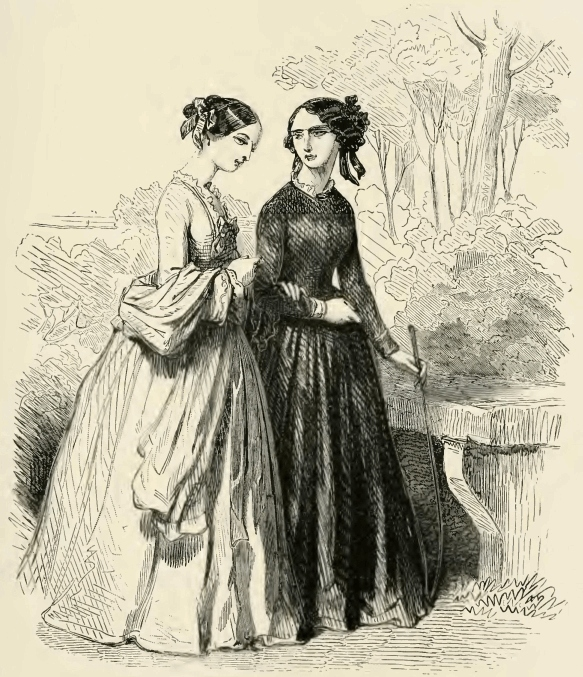
\includegraphics[width=\textwidth]{30151m.jpg}
\end{figure}

“Does Mademoiselle Danglars object to this marriage with M. de Morcerf
on account of loving another?”

“I told you I was not on terms of strict intimacy with Eugénie.”

“Yes, but girls tell each other secrets without being particularly
intimate; own, now, that you did question her on the subject. Ah, I see
you are smiling.”

“If you are already aware of the conversation that passed, the wooden
partition which interposed between us and you has proved but a slight
security.”

“Come, what did she say?”

“She told me that she loved no one,” said Valentine; “that she disliked
the idea of being married; that she would infinitely prefer leading an
independent and unfettered life; and that she almost wished her father
might lose his fortune, that she might become an artist, like her
friend, Mademoiselle Louise d’Armilly.”

“Ah, you see——”

“Well, what does that prove?” asked Valentine.

“Nothing,” replied Maximilian.

“Then why did you smile?”

“Why, you know very well that you are reflecting on yourself,
Valentine.”

“Do you want me to go away?”

“Ah, no, no. But do not let us lose time; you are the subject on which
I wish to speak.”

“True, we must be quick, for we have scarcely ten minutes more to pass
together.”

“\textit{Ma foi!}” said Maximilian, in consternation.

“Yes, you are right; I am but a poor friend to you. What a life I cause
you to lead, poor Maximilian, you who are formed for happiness! I
bitterly reproach myself, I assure you.”

“Well, what does it signify, Valentine, so long as I am satisfied, and
feel that even this long and painful suspense is amply repaid by five
minutes of your society, or two words from your lips? And I have also a
deep conviction that heaven would not have created two hearts,
harmonizing as ours do, and almost miraculously brought us together, to
separate us at last.”

“Those are kind and cheering words. You must hope for us both,
Maximilian; that will make me at least partly happy.”

“But why must you leave me so soon?”

“I do not know particulars. I can only tell you that Madame de
Villefort sent to request my presence, as she had a communication to
make on which a part of my fortune depended. Let them take my fortune,
I am already too rich; and, perhaps, when they have taken it, they will
leave me in peace and quietness. You would love me as much if I were
poor, would you not, Maximilian?”

“Oh, I shall always love you. What should I care for either riches or
poverty, if my Valentine was near me, and I felt certain that no one
could deprive me of her? But do you not fear that this communication
may relate to your marriage?”

“I do not think that is the case.”

“However it may be, Valentine, you must not be alarmed. I assure you
that, as long as I live, I shall never love anyone else!”

“Do you think to reassure me when you say that, Maximilian?”

“Pardon me, you are right. I am a brute. But I was going to tell you
that I met M. de Morcerf the other day.”

“Well?”

“Monsieur Franz is his friend, you know.”

“What then?”

“Monsieur de Morcerf has received a letter from Franz, announcing his
immediate return.” Valentine turned pale, and leaned her hand against
the gate.

“Ah heavens, if it were that! But no, the communication would not come
through Madame de Villefort.”

“Why not?”

“Because—I scarcely know why—but it has appeared as if Madame de
Villefort secretly objected to the marriage, although she did not
choose openly to oppose it.”

“Is it so? Then I feel as if I could adore Madame de Villefort.”

“Do not be in such a hurry to do that,” said Valentine, with a sad
smile.

“If she objects to your marrying M. d’Épinay, she would be all the more
likely to listen to any other proposition.”

“No, Maximilian, it is not suitors to which Madame de Villefort
objects, it is marriage itself.”

“Marriage? If she dislikes that so much, why did she ever marry
herself?”

“You do not understand me, Maximilian. About a year ago, I talked of
retiring to a convent. Madame de Villefort, in spite of all the remarks
which she considered it her duty to make, secretly approved of the
proposition, my father consented to it at her instigation, and it was
only on account of my poor grandfather that I finally abandoned the
project. You can form no idea of the expression of that old man’s eye
when he looks at me, the only person in the world whom he loves, and, I
had almost said, by whom he is beloved in return. When he learned my
resolution, I shall never forget the reproachful look which he cast on
me, and the tears of utter despair which chased each other down his
lifeless cheeks. Ah, Maximilian, I experienced, at that moment, such
remorse for my intention, that, throwing myself at his feet, I
exclaimed,—‘Forgive me, pray forgive me, my dear grandfather; they may
do what they will with me, I will never leave you.’ When I had ceased
speaking, he thankfully raised his eyes to heaven, but without uttering
a word. Ah, Maximilian, I may have much to suffer, but I feel as if my
grandfather’s look at that moment would more than compensate for all.”

“Dear Valentine, you are a perfect angel, and I am sure I do not know
what I—sabring right and left among the Bedouins—can have done to merit
your being revealed to me, unless, indeed, Heaven took into
consideration the fact that the victims of my sword were infidels. But
tell me what interest Madame de Villefort can have in your remaining
unmarried?”

“Did I not tell you just now that I was rich, Maximilian—too rich? I
possess nearly 50,000 livres in right of my mother; my grandfather and
my grandmother, the Marquis and Marquise de Saint-Méran, will leave me
as much, and M. Noirtier evidently intends making me his heir. My
brother Edward, who inherits nothing from his mother, will, therefore,
be poor in comparison with me. Now, if I had taken the veil, all this
fortune would have descended to my father, and, in reversion, to his
son.”

“Ah, how strange it seems that such a young and beautiful woman should
be so avaricious.”

“It is not for herself that she is so, but for her son, and what you
regard as a vice becomes almost a virtue when looked at in the light of
maternal love.”

“But could you not compromise matters, and give up a portion of your
fortune to her son?”

“How could I make such a proposition, especially to a woman who always
professes to be so entirely disinterested?”

“Valentine, I have always regarded our love in the light of something
sacred; consequently, I have covered it with the veil of respect, and
hid it in the innermost recesses of my soul. No human being, not even
my sister, is aware of its existence. Valentine, will you permit me to
make a confidant of a friend and reveal to him the love I bear you?”

Valentine started. “A friend, Maximilian; and who is this friend? I
tremble to give my permission.”

“Listen, Valentine. Have you never experienced for anyone that sudden
and irresistible sympathy which made you feel as if the object of it
had been your old and familiar friend, though, in reality, it was the
first time you had ever met? Nay, further, have you never endeavored to
recall the time, place, and circumstances of your former intercourse,
and failing in this attempt, have almost believed that your spirits
must have held converse with each other in some state of being anterior
to the present, and that you are only now occupied in a reminiscence of
the past?”

“Yes.”

“Well, that is precisely the feeling which I experienced when I first
saw that extraordinary man.”

“Extraordinary, did you say?”

“Yes.”

“You have known him for some time, then?”

“Scarcely longer than eight or ten days.”

“And do you call a man your friend whom you have only known for eight
or ten days? Ah, Maximilian, I had hoped you set a higher value on the
title of friend.”

“Your logic is most powerful, Valentine, but say what you will, I can
never renounce the sentiment which has instinctively taken possession
of my mind. I feel as if it were ordained that this man should be
associated with all the good which the future may have in store for me,
and sometimes it really seems as if his eye was able to see what was to
come, and his hand endowed with the power of directing events according
to his own will.”

“He must be a prophet, then,” said Valentine, smiling.

“Indeed,” said Maximilian, “I have often been almost tempted to
attribute to him the gift of prophecy; at all events, he has a
wonderful power of foretelling any future good.”

“Ah,” said Valentine in a mournful tone, “do let me see this man,
Maximilian; he may tell me whether I shall ever be loved sufficiently
to make amends for all I have suffered.”

“My poor girl, you know him already.”

“I know him?”

“Yes; it was he who saved the life of your step-mother and her son.”

“The Count of Monte Cristo?”

“The same.”

“Ah,” cried Valentine, “he is too much the friend of Madame de
Villefort ever to be mine.”

“The friend of Madame de Villefort! It cannot be; surely, Valentine,
you are mistaken?”

“No, indeed, I am not; for I assure you, his power over our household
is almost unlimited. Courted by my step-mother, who regards him as the
epitome of human wisdom; admired by my father, who says he has never
before heard such sublime ideas so eloquently expressed; idolized by
Edward, who, notwithstanding his fear of the count’s large black eyes,
runs to meet him the moment he arrives, and opens his hand, in which he
is sure to find some delightful present,—M. de Monte Cristo appears to
exert a mysterious and almost uncontrollable influence over all the
members of our family.”

“If such be the case, my dear Valentine, you must yourself have felt,
or at all events will soon feel, the effects of his presence. He meets
Albert de Morcerf in Italy—it is to rescue him from the hands of the
banditti; he introduces himself to Madame Danglars—it is that he may
give her a royal present; your step-mother and her son pass before his
door—it is that his Nubian may save them from destruction. This man
evidently possesses the power of influencing events, both as regards
men and things. I never saw more simple tastes united to greater
magnificence. His smile is so sweet when he addresses me, that I forget
it ever can be bitter to others. Ah, Valentine, tell me, if he ever
looked on you with one of those sweet smiles? if so, depend on it, you
will be happy.”

“Me?” said the young girl, “he never even glances at me; on the
contrary, if I accidentally cross his path, he appears rather to avoid
me. Ah, he is not generous, neither does he possess that supernatural
penetration which you attribute to him, for if he did, he would have
perceived that I was unhappy; and if he had been generous, seeing me
sad and solitary, he would have used his influence to my advantage, and
since, as you say, he resembles the sun, he would have warmed my heart
with one of his life-giving rays. You say he loves you, Maximilian; how
do you know that he does? All would pay deference to an officer like
you, with a fierce moustache and a long sabre, but they think they may
crush a poor weeping girl with impunity.”

“Ah, Valentine, I assure you you are mistaken.”

“If it were otherwise—if he treated me diplomatically—that is to say,
like a man who wishes, by some means or other, to obtain a footing in
the house, so that he may ultimately gain the power of dictating to its
occupants—he would, if it had been but once, have honored me with the
smile which you extol so loudly; but no, he saw that I was unhappy, he
understood that I could be of no use to him, and therefore paid no
attention to me whatever. Who knows but that, in order to please Madame
de Villefort and my father, he may not persecute me by every means in
his power? It is not just that he should despise me so, without any
reason. Ah, forgive me,” said Valentine, perceiving the effect which
her words were producing on Maximilian: “I have done wrong, for I have
given utterance to thoughts concerning that man which I did not even
know existed in my heart. I do not deny the influence of which you
speak, or that I have not myself experienced it, but with me it has
been productive of evil rather than good.”

“Well, Valentine,” said Morrel with a sigh, “we will not discuss the
matter further. I will not make a confidant of him.”

“Alas!” said Valentine, “I see that I have given you pain. I can only
say how sincerely I ask pardon for having grieved you. But, indeed, I
am not prejudiced beyond the power of conviction. Tell me what this
Count of Monte Cristo has done for you.”

\begin{figure}[ht]
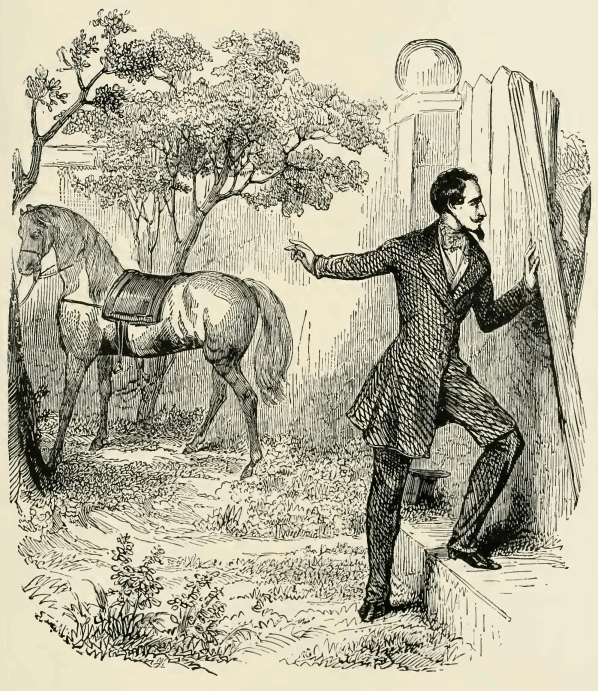
\includegraphics[width=\textwidth]{30157m.jpg}
\end{figure}

“I own that your question embarrasses me, Valentine, for I cannot say
that the count has rendered me any ostensible service. Still, as I have
already told you, I have an instinctive affection for him, the source
of which I cannot explain to you. Has the sun done anything for me? No;
he warms me with his rays, and it is by his light that I see
you—nothing more. Has such and such a perfume done anything for me? No;
its odor charms one of my senses—that is all I can say when I am asked
why I praise it. My friendship for him is as strange and unaccountable
as his for me. A secret voice seems to whisper to me that there must be
something more than chance in this unexpected reciprocity of
friendship. In his most simple actions, as well as in his most secret
thoughts, I find a relation to my own. You will perhaps smile at me
when I tell you that, ever since I have known this man, I have
involuntarily entertained the idea that all the good fortune which has
befallen me originated from him. However, I have managed to live thirty
years without this protection, you will say; but I will endeavor a
little to illustrate my meaning. He invited me to dine with him on
Saturday, which was a very natural thing for him to do. Well, what have
I learned since? That your mother and M. de Villefort are both coming
to this dinner. I shall meet them there, and who knows what future
advantages may result from the interview? This may appear to you to be
no unusual combination of circumstances; nevertheless, I perceive some
hidden plot in the arrangement—something, in fact, more than is
apparent on a casual view of the subject. I believe that this singular
man, who appears to fathom the motives of everyone, has purposely
arranged for me to meet M. and Madame de Villefort, and sometimes, I
confess, I have gone so far as to try to read in his eyes whether he
was in possession of the secret of our love.”

“My good friend,” said Valentine, “I should take you for a visionary,
and should tremble for your reason, if I were always to hear you talk
in a strain similar to this. Is it possible that you can see anything
more than the merest chance in this meeting? Pray reflect a little. My
father, who never goes out, has several times been on the point of
refusing this invitation; Madame de Villefort, on the contrary, is
burning with the desire of seeing this extraordinary nabob in his own
house, therefore, she has with great difficulty prevailed on my father
to accompany her. No, no; it is as I have said, Maximilian,—there is no
one in the world of whom I can ask help but yourself and my
grandfather, who is little better than a corpse—no support to cling to
but my mother in heaven!”

“I see that you are right, logically speaking,” said Maximilian; “but
the gentle voice which usually has such power over me fails to convince
me today.”

“I feel the same as regards yourself.” said Valentine; “and I own that,
if you have no stronger proof to give me——”

“I have another,” replied Maximilian; “but I fear you will deem it even
more absurd than the first.”

“So much the worse,” said Valentine, smiling.

“It is, nevertheless, conclusive to my mind. My ten years of service
have also confirmed my ideas on the subject of sudden inspirations, for
I have several times owed my life to a mysterious impulse which
directed me to move at once either to the right or to the left, in
order to escape the ball which killed the comrade fighting by my side,
while it left me unharmed.”

“Dear Maximilian, why not attribute your escape to my constant prayers
for your safety? When you are away, I no longer pray for myself, but
for you.”

\begin{figure}[ht]
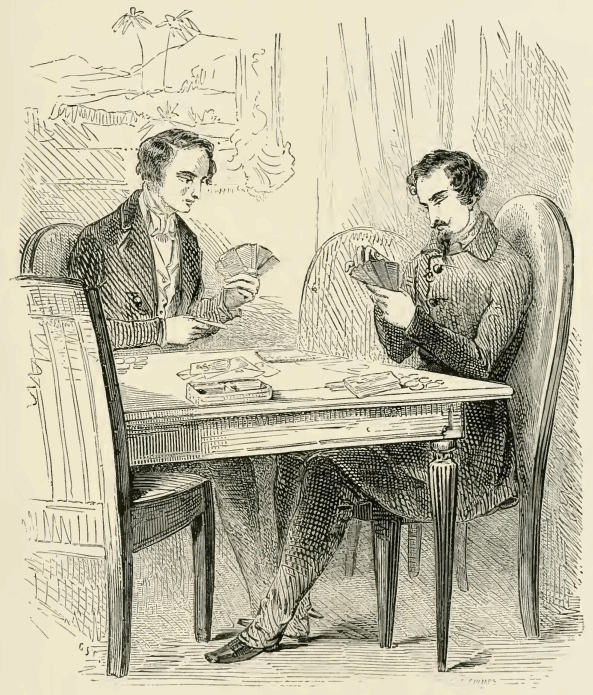
\includegraphics[width=\textwidth]{30159m.jpg}
\end{figure}

“Yes, since you have known me,” said Morrel, smiling; “but that cannot
apply to the time previous to our acquaintance, Valentine.”

“You are very provoking, and will not give me credit for anything; but
let me hear this second proof, which you yourself own to be absurd.”

“Well, look through this opening, and you will see the beautiful new
horse which I rode here.”

“Ah! what a beautiful creature!” cried Valentine; “why did you not
bring him close to the gate, so that I could talk to him and pat him?”

“He is, as you see, a very valuable animal,” said Maximilian. “You know
that my means are limited, and that I am what would be designated a man
of moderate pretensions. Well, I went to a horse dealer’s, where I saw
this magnificent horse, which I have named Médéah. I asked the price;
they told me it was 4,500 francs. I was, therefore, obliged to give it
up, as you may imagine, but I own I went away with rather a heavy
heart, for the horse had looked at me affectionately, had rubbed his
head against me and, when I mounted him, had pranced in the most
delightful way imaginable, so that I was altogether fascinated with
him. The same evening some friends of mine visited me,—M. de
Château-Renaud, M. Debray, and five or six other choice spirits, whom
you do not know, even by name. They proposed a game of \textit{bouillotte}. I
never play, for I am not rich enough to afford to lose, or sufficiently
poor to desire to gain. But I was at my own house, you understand, so
there was nothing to be done but to send for the cards, which I did.

“Just as they were sitting down to table, M. de Monte Cristo arrived.
He took his seat amongst them; they played, and I won. I am almost
ashamed to say that my gains amounted to 5,000 francs. We separated at
midnight. I could not defer my pleasure, so I took a cabriolet and
drove to the horse dealer’s. Feverish and excited, I rang at the door.
The person who opened it must have taken me for a madman, for I rushed
at once to the stable. Médéah was standing at the rack, eating his hay.
I immediately put on the saddle and bridle, to which operation he lent
himself with the best grace possible; then, putting the 4,500 francs
into the hands of the astonished dealer, I proceeded to fulfil my
intention of passing the night in riding in the Champs-Élysées. As I
rode by the count’s house I perceived a light in one of the windows,
and fancied I saw the shadow of his figure moving behind the curtain.
Now, Valentine, I firmly believe that he knew of my wish to possess
this horse, and that he lost expressly to give me the means of
procuring him.”

“My dear Maximilian, you are really too fanciful; you will not love
even me long. A man who accustoms himself to live in such a world of
poetry and imagination must find far too little excitement in a common,
every-day sort of attachment such as ours. But they are calling me. Do
you hear?”

“Ah, Valentine,” said Maximilian, “give me but one finger through this
opening in the grating, one finger, the littlest finger of all, that I
may have the happiness of kissing it.”

“Maximilian, we said we would be to each other as two voices, two
shadows.”

“As you will, Valentine.”

“Shall you be happy if I do what you wish?”

“Oh, yes!”

Valentine mounted on a bench, and passed not only her finger but her
whole hand through the opening. Maximilian uttered a cry of delight,
and, springing forwards, seized the hand extended towards him, and
imprinted on it a fervent and impassioned kiss. The little hand was
then immediately withdrawn, and the young man saw Valentine hurrying
towards the house, as though she were almost terrified at her own
sensations.
